\RequirePackage{etex}
\documentclass[10pt,onecolumn,twoside,openany,bg=full,layout=true]{dndbook}

% Use babel or polyglossia to automatically redefine macros for terms
% Armor Class, Level, etc...
% Default output is in English; captions are located in lib/dndstring-captions.sty.
% If no captions exist for a language, English will be used.
%1. To load a language with babel:
%	\usepackage[<lang>]{babel}
%2. To load a language with polyglossia:
%	\usepackage{polyglossia}
%	\setdefaultlanguage{<lang>}
\usepackage[english]{babel}
%\usepackage[czech]{babel}
% For further options (multilanguage documents, hypenations, language environments...)
% please refer to babel/polyglossia's documentation.
\usepackage[utf8]{inputenc}
\usepackage[singlelinecheck=false]{caption}
\usepackage{lipsum}
\usepackage{listings}
\usepackage{shortvrb}
\usepackage{wrapfig}
\usepackage{enumerate}
\usepackage{graphicx}
\usepackage[colorlinks = true,
            linkcolor = blue,
            urlcolor  = blue,
            citecolor = blue,
            anchorcolor = blue,
            urlbordercolor = blue,
            pdfborderstyle={/S/U/W 1}]{hyperref}
\usepackage{parskip}
\usepackage{pdfpages}

%\hypersetup{
%    colorlinks=true,
%    linkcolor=blue,
%    filecolor=magenta,
%    urlcolor=cyan,
%    }



%\captionsetup[table]{labelformat=empty,font={sf,sc,bf,},skip=0pt}

\MakeShortVerb{|}

\lstset{
  basicstyle=\ttfamily,
  language=[LaTeX]{TeX},
  breaklines=true,
}

\begin{document}
\frontmatter
\title {Convicts' Quest\\ \large TTRPG Adventure set in Forgotten Realms}
\author {by: Tomáš Fanta}
\date {2024}



\begin{titlepage}
    \centering
    \textbf {\huge Convicts' Quest\\\large TTRPG Adventure set in Forgotten Realms\\}
    \textbf {Tomáš Fanta\\}
    \textbf {2024\\}
    \vspace{1.5cm}
    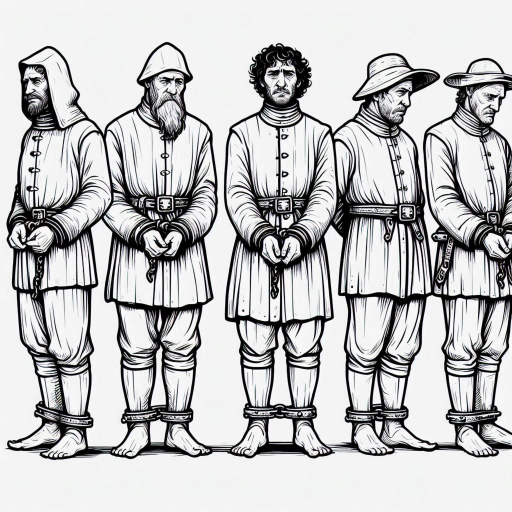
\includegraphics[width=0.5\textwidth]{img/title}\\[1cm]
    \vfill
    \begin{flushleft}
      \footnotesize
      This adventure, text documents and other materials are inspired or adapted from the following sources:

      - Waterdeep: Dragon Heist, 5th Edition, Wizards of the Coast.
      - Forgotten Realms lore, 5th Edition, Wizards of the Coast.
      - DnD 5e Player's Handbook, Dungeon Master's Guide, Monster Manual, Wizards of the Coast.

      All copyrights and trademarks are owned by their respective owners.

      This is a fan-made adventure, that serves for non-commercial use, and I am not affiliated with Wizards of the Coast.

      This document is provided "as is" without warranty of any kind, either express or implied, including, but not limited to,
      the implied warranties of merchantability and fitness for a particular purpose.
      The entire risk as to the quality and performance of the document is with you.
      Should the document prove defective, you assume the cost of all necessary servicing, repair or correction.

      Convicts' Quest © 2024 by Tomáš Fanta is licensed under CC BY-NC-ND 4.0. To view a copy of this license, visit \texttt{https://creativecommons.org/licenses/by-nc-nd/4.0/}
    \end{flushleft}
\end{titlepage}


\tableofcontents

\mainmatter

\twocolumn
\chapter{Introduction}\label{ch:introduction}
\DndDropCapLine{T}{his adventure is designed as introduction to DnD}
which could be enjoyed both by beginners and experienced players.
For the DMs it is expected to have some experience with DnD 5e rules and Forgotten Realms setting.

The duration may vary depending on players' pace and experience.
During my testing with two different groups, it took around 4-6 hours to finish the adventure.

The adventure is designed for 3 players with characters of 2nd level (and one DM).

It is expected for the DM to mix and adapt the adventure to the players' actions and choices.

Please note that this is a fan-made adventure, that serves for non-commercial use, I am the author of the characters,
the story and the maps.
The rest of the content is based on the DnD 5e rules and ForgottenRealms setting and adventure Waterdeep: Dragonheist, but it can be easily adapted to other
settings and TTRPG rules.

Creature statistics, spells, character sheets and Trollskull mansion map design (not the image itself) are taken from DnD 5e materials,
and it is expected that the DM has access to them if they intend to use them.


\subsection*{Adventure theme}
Sandbox urban fantasy with slight vampiric influence, following the classic conflict between criminal and ruling forces,
centred particularly on cooperative storytelling with classic elements of dungeon crawling, political intrigue, light settlement building, and exploration.

\subsection*{Narative pitch}
The group of convicts who have just served their sentence of forced labour in the metropolis of Waterdeep on the shores of the Sword Coast,
attempting to cleanse their names, pay off debts, and perhaps join the elite group of adventurers who protects the city.
However, the journey will be arduous, filled with constant conflicts between the criminal underworld and city forces.
But a new player enters the scene with a growing community vying for the position of the masked lord.
The choice is yours on whom to support to achieve your goals.

\subsection*{The tone and aim of the game}
Aim for more serious cooperative storytelling, focused more on RP than on combat.
Important thing is to have fun together.

  \begin{DndComment}{General tips to make your game more enjoyable}
    \begin{itemize}
      \item \textbf{Rule of discussion} - Everyone tries to ensure that everyone speaks for the same amount of time.
      \item \textbf{Cooperation} - DM is not playing against the players but with them.
      \item \textbf{Don't argue with DM} - If you disagree with the DM, discuss it after the game.
      \item \textbf{Do not metagame} - Do not use out-of-game knowledge in-game.
      \item \textbf{Do not cheat} - The game is about fun, not winning.
      \item \textbf{Talk in character} - It's more immersive.
      \item \textbf{Focus on the game} - take breaks if needed, set-up do-not-disturb mode.
      \item \textbf{Improvisation} - DM doesn't know everything so expect some improvisation.
    \end{itemize}
  \end{DndComment}
\vfill
\pagebreak

\onecolumn
\chapter{Player characters}\label{ch:player-characters}
\section{Choosing a character}\label{sec:choosing-a-character}
Let players choose from these premade characters or create their own.
This is also an information everyone knows about each other.
If players choose to create their own characters, they should be from around Waterdeep and have been on forced labour with others.
They should have
After they choose, give them full backstory which includes character's secrets.

%\vfill
%\newpage

\section{Premade characters}\label{sec:premade-characters}
  \begin{wrapfigure}{r}{0.2\textwidth}
    \begin{center}
      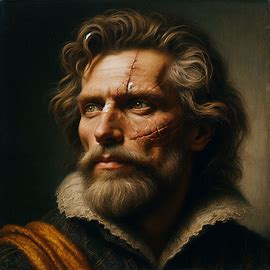
\includegraphics[width=0.2\textwidth]{img/characters/harold}
    \end{center}
  \end{wrapfigure}
  \subsection {Harold "Scar" of Kremle}\label{subsec:harold-"scar"-of-kremle}
\paragraph{Heavy weapons fighter}
Despite being a lyricist, he has an unusually muscular build and strong arms, almost as if the small instrument in his
hand might accidentally be crushed.\par
Clearly familiar with both the city and the wilderness, hard work is no stranger to him.\par
An ugly scar on his face gives him a rather intimidating expression more fitting for a criminal than a wandering bard,
even though his attire and rather joyous expression might suggest otherwise.

  \begin{wrapfigure}{r}{0.2\textwidth}
    \begin{center}
      
\includegraphics[width=0.2\textwidth]{img/characters/yasmina}
    \end{center}
  \end{wrapfigure}
  \subsection{Yasmina}\label{subsec:yasmina}
  \paragraph{Divination Wizard}
  An enthusiastic human wizard, longing for adventure, who always wears a diadem on her forehead.\par
  She claims to have done forced labour because she refused a powerful lecherous nobleman, and her lawyer messed it up,
  turning her from a victim into a perpetrator.\par
  She seems to be very clever, not ugly either, and moves as gracefully as a cat, but they've never entrusted her
  with anything heavier than a broom.\par
  She is knowledgeable in history and magic and has occasionally saved someone from injury thanks to her visions.

  \begin{wrapfigure}{r}{0.2\textwidth}
    \begin{center}
      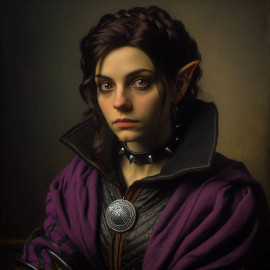
\includegraphics[width=0.2\textwidth]{img/characters/silgrid}
    \end{center}
  \end{wrapfigure}
  \subsection{Silgrid Coalbraid}\label{subsec:silgrid-coalbraid}
  \paragraph{Dwarven rogue} A trusting, devout dwarf with a dark metal collar.
  She exudes compassion and understanding, but she might be a bit of a weirdo; I feel like she experiences other
  people's emotions too intensely.
  Unlike other dwarves, she's rather small and slender, probably wouldn't last long
  in the mines, but she moves quickly and has a good aim.
  She often discreetly prays in dark alleys when nobody's looking.
  She always wears a dark clothes, and despite all her strange quirks, she's quite easy to talk to.

  \begin{wrapfigure}{r}{0.2\textwidth}
    \begin{center}
      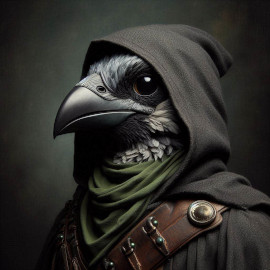
\includegraphics[width=0.2\textwidth]{img/characters/sally}
    \end{center}
  \end{wrapfigure}
  \subsection{Sally “Jackdaw” Horst}\label{subsec:sally-jackdaw-horst}
  \paragraph{Kenku ranger, druid fighting style}
  A secretive grey-black Kenku rumoured to have once been part of the city watch.
  Unable to speak, only mimics other voices and sounds.
  Not very strong, which isn't unusual for a bird-like race.
  Appears to act with caution and not be overly swayed by emotions.
  Moves calmly and carefully observes the surroundings, alert to every rustle.
  Seems to have a grasp of nature and remains unfazed by anything in the city.
  He values morality highly and despises all criminal activities.

\vfill

\chapter{Character backstories}\label{ch:character-backstories}
\section{Harold "Scar" of Kremle}\label{sec:harold-"scar"-of-kremle}
\subsection{Backstory}\label{subsec:harold-backstory}
\begin{wrapfigure}{r}{0.4\textwidth}
  \begin{center}
    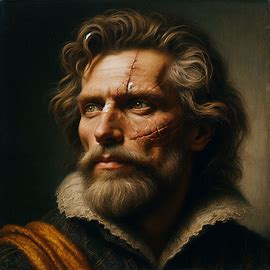
\includegraphics[width=0.4\textwidth]{img/characters/harold}
  \end{center}
\end{wrapfigure}
Harold was born in the forest village of Kremle, to a hunter's wife.
He spent most of his childhood in the woods with his father, who taught him everything about nature, survival, and hunting.
In his teens, he yearned to experience life in the city, which his father so despised.
He spent most of his free time in the taverns of the nearby small town of Grapewade,
where he unsuccessfully tried to perform as a solo lyrist, hoping to travel the world as a wandering bard.
Due to criticism in the tavern, he often got into fights, and once he got slashed by a broken bottle to the face.
Since then, they called him nothing but "Scar".

Despite not being naturally endowed with beauty or charisma, he ventured into the metropolis of Waterdeep, after a
a heated argument with his Firbolg girlfriend, Iskrenost, from whom he learned the language of giants.

In Waterdeep, he failed as a bard, and to make a living, he started doing what he knew best - hunting.
But his prey were not animals, but mostly criminals.
He lived in the city and hunted people or other beings, spending his spare time in taverns or with esteemed music teachers.

On the way of becoming a better lyre player he was the one being played, by his rival.
Envious human bounty hunter named Ray Cox tricked him into kidnapping an innocent woman and
reported him to the city watch.\par
Harold was sentenced to a year of forced labour and a ban on bounty hunting for an additional year.
Now, after serving his sentence, Harold was banned to do his dirty trade, and the only more
lucrative option to afford teachers and finally achieve fame as a musician is to become an adventurer.
\subsubsection{Secrets}
  \begin{itemize}
    \item He conceals his past as a bounty hunter
    \item He was pretending to be a musician, although he was not very good at it (even after years, he still made mistakes).
    \item He certainly lacks bardic abilities but tries to socialize as a typical bard would.
  \end{itemize}

\vfill
\pagebreak


\section{Yasmina}\label{sec:yasmina}
\subsection{Backstory}\label{subsec:yasmina-backstory}
\begin{wrapfigure}{r}{0.4\textwidth}
  \begin{center}
    
\includegraphics[width=0.4\textwidth]{img/characters/yasmina}
  \end{center}
\end{wrapfigure}
Born as an unwanted child of a sea elf mercenary and a human sorceress who studied marine magical phenomena on the
island of Mintarn near the Sword Coast.
Shortly after birth, her father disowned her, and with her mother, she sailed
to Neverwinter, where she spent most of her childhood.

Her mother was ashamed of her romance with Yasmina's father, so she disguised her daughter.
To conceal her origin, she created an enchanted diadem that adjusted the shape of her ears, concealed her gills,
and changed the colour of her skin from green-blue to a human fair complexion.

Magic ran in her blood, and she learned everything she could from her mother and later from private tutors at the
House of Knowledge.
Because of her mother's influence, she distrusted men, especially elves, travellers, adventurers, and mercenaries.

Her talent for divination magic manifested during puberty, and she began to exploit it as much as she could.
In dubious ventures, she posed as a wealthy merchant, winning bets thanks to her limited knowledge of the future.
She was exposed by an older tiefling woman named Larsa, who blackmailed her into smuggling magical items and
participating in various scams.
Before Larsa was imprisoned for organizing an illegal cult worshipping demonic forces, Yasmina managed to learn
everything from her and also express unrequited love for her.
When she confessed to her mother what she had got herself into, she was thrown out of the house.

Using magic and deception, Yasmina managed to acquire a wagon and a donkey and set out southward.
She read fortunes for travellers and mocked, tricked and swindled arrogant adventurers, mercenaries, or soldiers,
but tried to help the poor and women.

In the city of Waterdeep, she completely succumbed to her hobby of disguising and deceiving people.
She got into debt, bought all the necessary luxury clothing and accessories, forged documents, and began to impersonate
a local noblewoman to acquire her estate and a comfortable life.
In the end, she took too much risk and offended an influential man (Arnold Klinger), who uncovered her disguise.
She very unpleasantly bribed the lecherous judge Methodius, and instead of whipping and imprisonment,
she had to do forced labour for a year.

All she had left was a magical diadem, her personal belongings, and a hefty debt (500 gold) to a loan shark named "Goldsmith."

She decided to take a break from illegal activities and reluctantly admitted that the only way to make big money was
to become an adventurer.
She disguised herself as an enthusiastic wizard who craved adventure.

\subsubsection{Secrets}\label{subsec:yasmina-secrets}
\begin{itemize}
\item She conceals her fraudulent past as well as her racial identity she is ashamed of.
\item She poses as an enthusiastic wizard while, in reality, she is cynical and greedy.
\item The only ones she cares about are women in distress and the poor, but she also tries to hide that,
this might be the only thing which would make her become an honest good person.
\end{itemize}

\vfill
\pagebreak

\section{Silgrid Coalbraid}\label{sec:silgrid-coalbraid}
\subsection{Backstory}\label{subsec:silgrid-backstory}
\begin{wrapfigure}{r}{0.4\textwidth}
  \begin{center}
    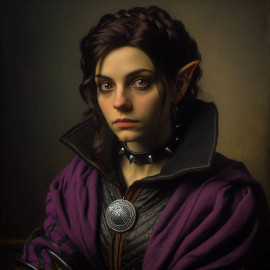
\includegraphics[width=0.4\textwidth]{img/characters/silgrid}
  \end{center}
\end{wrapfigure}

Born in the Troll Mountains in an underground settlement of gold and shield dwarves.
The settlement often faced attacks from drow and goblins, resulting in the deaths of many of her clanmates and friends,
leading her to become apathetic and suppress all grief within herself.
She limited her contact with others and immersed herself in her destructive craft - mining alchemy.


The population of the settlement decreased so much that the council of elders decided to destroy the village and mines
and seek refuge in the nearby trade city of Easting.

Feeling lonely and full of unexpressed sorrow in a foreign city on the surface, Silgrid succumbed to the preaching and
manipulations of Nemio, the leader of the local secret sect of the goddess of loss and darkness, Shar.
In the underground hideout, she trained and served as a scout and soldier for the cult.
She prayed to forget the suffering of her clanmates and the loss of her home.
The pounding on the stone gate, calling for help, the roar of Rhûn, her love, when a horde of goblins overwhelmed him.
But blessings did not come, and she believed that only through devoted service could she gain the favour of the goddess Shar.
At the command of Nemio, she slew many, including goblins and fanatics trying to suppress freedom of worship.

She eventually processed her emotions and adopted a new outlook on the world.
She argued that loss is a great opportunity for a new and better beginning and that without darkness there is no light.
For her overly positive views on loss and darkness and her desire to help others cope with their loss,
she was labelled a heretic and banished.

Furious, Nemio, the high priestess, had her whipped as a farewell gesture left her only with a modest black garment
and placed a cursed black iron collar on her.

She took exile as a new beginning and an opportunity to help.
However, the curse of the collar soon manifested, and she experienced the suffering of the people she encountered in her dreams.

In Waterdeep, she sought ways to remove the collar.
She believed that with the help of magic, it could be done.
She had no access to mage services, so she "borrowed" a magical wand from one wizard named Forts.
However, the wand did not break the collar, and in a weak moment, Silgrid went to apologize and return the wand,
intoxicated by a strong dose of liquor.
The offended mage immediately summoned the city guard, and it wasn't long before the dwarf was performing forced labour
and had a debt of 200 gold pieces for the fine.

After a year of suffering, she decided to try something more honourable and decided to seek work as an adventurer
to pay off her debt and perhaps meet a mage who could help her remove the collar.

\subsubsection{Secrets}
\begin{itemize}
  \item Former cultist
  \item A black iron collar that cannot be removed
  \begin{itemize}
    \item The character strongly empathizes with the sorrow, suffering, and depression of characters within a 5-foot radius
  \end{itemize}
\item Worships Shar
\end{itemize}

\vfill
\pagebreak


  \section{Sally "Jackdaw" Horst}\label{sec:sally-jackdaw-horst}
  \subsection{Backstory}\label{subsec:sally-backstory}
  \begin{wrapfigure}{r}{0.4\textwidth}
    \begin{center}
      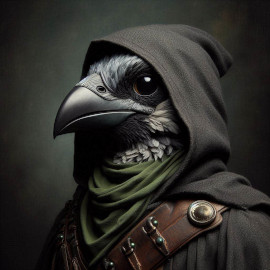
\includegraphics[width=0.4\textwidth]{img/characters/sally}
    \end{center}
  \end{wrapfigure}

He was born as a human into a family of a kind merchant dealing in glass and ceramics, located on the border between the
commercial and port districts of the city of Waterdeep.
When he was little, his parents took in an orphan who had tried to steal from their shop, so Sally suddenly had an
older brother.
Throughout their childhood, they engaged in innocent mischief and explored every corner of the city.

As Sally began perceiving criminal elements' influence on the city, he desired to change the situation.
He studied at the military academy and joined the city watch, eventually rising to the rank of investigator.

During the investigation of the disappearance of children in the impoverished district, he believes an unknown entity
cursed him.
He began to transform into an avian form until he appeared like a grey-black feathered Kenku.
With this transformation, he gained natural magical abilities and the natural skills of Kenkus, losing his ability
to speak.

After the transformation, he occasionally lost consciousness and woke up with bloody talons,
hearing a bird-like voice in his head.
He discovered that he hunted criminals at night, using his newfound skills.
When his nocturnal activities were discovered, he received a symbolic mild punishment—a year of forced labour and
expulsion from the city guard.

During his sentence, his brother Larry fell ill and could no longer manage his work as a merchant,
which Sally took over from his father.
Sally has a desire to help his brother and will financially support him if possible.

Becoming an adventurer was a clear choice for him—a chance for great wealth, doing good deeds, and the opportunity to
explore and master his animalistic self.

\subsubsection{Secrets}
\begin{itemize}
  \item The human investigator's origin
  \item Crimes committed on criminals, subconsciously during his uncontrolled transformation
  \item Voice in his head which he hears after losing control
  \item He believes he is cursed, but he knows very little about it
\end{itemize}

\vfill
%\pagebreak

\chapter{Adventure}\label{ch:adventure}
Let the players read their sheets and backstories and get familiar with it.
Allow them to specify their appearance if they want to.

You as a DM pick one of the premade characters, whichever is left or create your own character to play with them as a fellow convict and
friend.
Role of this NPC is to guide the players, let's call this NPC "Norman", friendly bagpiper, tavern brawler who has a story for every situation.
It is important that this NPC is their friend who served the sentence with them and should have strong relationship with them.

Tell players to share their secrets in character gradually during the game, when they feel it's appropriate or as a DM use
NPCs to ask questions to help expose their secrets during RP (don't force it).
This may help to create a more immersive experience, if you feel there's some empty moment or during a rest.

Agree on rules and answer any questions players might have.

You're ready to begin.

\newcounter{act_num}
\setcounter{act_num}{1}

\section{Act \roman{act_num}}\label{sec:act-roman{act_num}}
\addtocounter{act_num}{1}

\newcounter{subact_num}
\setcounter{subact_num}{1}
\subsection{\arabic{subact_num} - Forced Labour Control Bureau}\label{subsec:\arabic{subact_num}-forced-labour-control-bureau}
\addtocounter{subact_num}{1}

Start with reading the following text aloud to the players (everything in this box is meant to be read aloud further on):
\begin{DndReadAloud}
\begin{itemize}
\item A damp and cool feeling typical of a dungeon creeps into the nose.
The noise of the big city during the hot summer is very muffled on the ground floor in the stone building of the Forced Labour Control Bureau.
But the speech of bald old Magister in black robes about how to behave correctly cannot be overheard.
\item You already have your civilian clothes on, you don't have to build anything, carry anything, clean the streets,
serve the nobility or farm.
It's been a long year...
\item The man behind the desk continues:
"Your sentence is hereby served, now please all sign here one by one."
\item The bald man gradually starts to call out by name.
\end{itemize}
\end{DndReadAloud}

And the players gradually begin to describe their characters as they are called out.
Start with most confident player or choose your NPC and describe them yourself.
Then let the players describe their characters and sign the papers.
\begin{DndReadAloud}
After everyone signs the man continues:
"Oh, Silgrid Coalbraid, your debt is 200 gold pieces, due by next month."
"That's all, I hope I don't see you here again.
  Thanks for your work and good luck!"
  After that, the clerk will signal you to go outside.
"Wait a minute, I just remembered, if you want some honest work, we are now hiring people to exterminate rats in warehouses and sewers!"
You all go out to a small square.
You can see a marble palace and a high tower opposite of you, and further to the south you catch a glimpse of Mount Waterdeep with a giant statue of a Griffin on top.
\end{DndReadAloud}
Let the players RP and chat (in character) in front of the office building.
Norman will give suggestions and role-play prompts if players are stuck:
\begin{itemize}
  \item Silgrid, don't you want to buy some armour?
  \item How do we start our adventurous career?
  \item Forced labour was enough for me, I don’t want to do anything illegal any more, what about you?
  \item Killing rats in warehouses and sewers - ugh, no!
  \item Do we jump straight into the Yawning Portal?
  \begin{itemize}
    \item I have one contact there.
  \end{itemize}
\end{itemize}
\begin{DndReadAloud}
"Come on, I can't wait to go on an adventure!" Norman declares.
\end{DndReadAloud}
Let players make an Insight roll (as Norman attempts to deceive them with DC 10).
\begin{itemize}
\item Rolls above 10 you can tell players that Norman is hiding something, but it's not clear what.
\item Otherwise, they don't notice anything.
\end{itemize}
In reality Norman can't wait to go to a tavern and drink to celebrate his freedom.


If players decide to go back to the clerk, about the job offer, he will tell them that the job is not very well paid (1g each per night of de-ratization), but it's honest work.
You have to improvise here, montage the rat slaying, simply describe it, or you can prepare a small encounter with rats in a warehouse or sewers.

\subsection{\arabic{subact_num} - To the Yawning Portal}\label{subsec:\arabic{subact_num}-to-the-yawning-portal}
\addtocounter{subact_num}{1}
Norman will lead the group to the Yawning Portal pub (~15min walk south-west, in front of Waterdeep Castle, in Castle Ward).
\begin{DndReadAloud}
As you walk through the city, the streets are packed with all kinds of people of various races.
Air is hot, you hear the shouts of vendors, smell of a thousand different foods cooking and the stench of the streets and the port mixing into a typical crowded city chaos.
\end{DndReadAloud}

As they walk the crowded street, ask them to roll perception check (DC 10) or just use their passive perception or
tell describe the following to the character with the highest perception:
\begin{DndReadAloud}
\paragraph{ To high preception character}
  You noticed a hooded figure trying to grab Yasmina's hand, whispering something to her ear and then quickly tries to disappear in the crowd.
\end{DndReadAloud}
Do not tell other players what it is exactly, let Yasmina's player decide if she wants to share it with others.
\begin{DndReadAloud}
\paragraph{ To Yasmina only}
Going through the crowded street, a hooded figure tries to grab your hand and says in a gruff voice:
"You owe 500 gold to The Goldsmith , you have a tenday.
  Don't try to run away.
  Bring it to Undercliff."
  And the figure quickly disappears into the crowd.
\end{DndReadAloud}
Players may role-play the situation or interact with the figure, but the person will not respond and if further harassed they'll try to call the city watch.

\begin{DndReadAloud}
As you are approaching the tavern you see city watch patrol catching a thief right on the street, and they shout: "Magister!".
Within a moment a man in a black robe appears and soon pronounces the verdict on the culprit and leads him towards the
nearest city watch station, from where whip blows and screams can be heard as you go around.
\end{DndReadAloud}
(If Silgrid is around she will experience the torment of the thief.)

\begin{DndReadAloud}
You reach the Yawning Portal and even in the morning there are quite a few guests - adventurers,
someone is descending into the 40-foot-diameter well in the middle of the tavern using rope-and-pulley mechanism.
The people sitting around are laughing and betting.
Nearby, a bald dark-skinned female cleric with golden jewellery is treating a wounded halfling.
\end{DndReadAloud}
(Again if Silgrid is around she will experience the pain of the wounded halfling.)
\vfill
\newpage

\section{Act \roman{act_num}}\label{sec:act-\roman{act_num}}
\addtocounter{act_num}{1}

\subsection{Opportunities}\label{subsec:opportunities}
Norman will lead the group to a table and order a round of drinks then leave to find his contact within the tavern.

You can give players following options to choose from, but as default I suggest to start with Lyra's plea, others can be omitted.
If you'd notice players thirst for combat you can start with the "Swarm of bats".

\subsubsection{Lyra's plea}
\begin{DndReadAloud}
  While enjoying a drink.
  A richly dressed young lady approaches your table.
  With desperate expression on her face, she says:
  "Greetings, my name's Lyra Lessoir, I need your help!"
  As she begins to explain, she sits at Norman's chair.
\end{DndReadAloud}
Improvise the conversation.
Lyra will ask the group to help her find her father who went to Undermountain and hasn't returned yet.
She offers 500 gold to bring her father (alive).
Lyra describes him as sixty-year old man with a grey beard and short hair, wearing a breastplate with a family crest and a scimitar with a blue gemstone in the hilt.
Lyra lends the group her mother's ring which is showing the way to the secret door within the Undermountain's dungeon level.
She explains that her father's crew used to go through the concealed door to their fortune hunting expeditions.
During the conversation with Lyra, another person comes to their table.
A man in a black and yellow "Landsknecht" outfit with red accessories and a twirled moustache.
He heard the Lyra's plea for help and brazenly offers to take it.
Harold (or one of the players of your choosing) recognizes him as his rival - Ray Cox.
The mercenary will boast and tries to persuade the lady that "these guys can't handle it".
Lyra will say that she will be waiting here or at her mansion in the Sea Ward (Lessoir Mansion).

\subsubsection{Norman's contact}
\begin{DndReadAloud}
  Norman returns to the table with a middle-aged man (brown hair cut by a pot) with sleepy eyes and brown tight-fit tailored clothes.

  "This is my contact I told you about, Arnold; he has a job for us."

  Arnold bows slightly and says:
  "Greetings, I am Arnold Fenxis, I need someone to walk through a building and make sure it's safe and clear of any potential unwanted guests.
  It should be fairly simple task.
  I can offer you 50 gold pieces for this job."

  "On another note, I overheard the conversation with the lady, and If you happen to find any loot on the way to save her father, I can offer you a fair price for it.
  If you decide to take the job."
\end{DndReadAloud}
He's interested in buying the house from the city (soon to be forfeited to the city as probate expires), but he needs to make sure it's safe first.
House is supposed to be haunted, but he doesn't believe in ghosts.
He usually drinks at the Yawning Portal, or you can leave a message with Durnan (the barkeep).

\subsubsection{Swarm of bats}
If players refuse all the quests and nothing is happening for a long time three
\href{https://www.dndbeyond.com/monsters/17028-swarm-of-bats}{swarm of bats} start terrorizing the pub coming from the well in the middle of the room.

When the bats are defeated, Durnan the barkeep will ask the group to down the well and task them to close the door at bottom of the as someone left it open (for 5g).
At the bottom of the well there is a room with four reinforced doors and a levers to close them, one of those were left open - pulling a lever will close it.
\vfill
\newpage

\subsection{Lyra's plea}\label{subsec:lyras-plea}
Characters have to pay 1 gold each to descend into the well on a pulley.
It's 140ft deep, and it takes ~10 minutes to descend.
At the bottom, they find a room with four reinforced doors and a lever to open them.
Lyra's ring has some kind of magical arrow on it pointing towards a direction like a compass.
It points to the west door.
\subsubsection{Going through the dungeon level}
You can share the following information with the players or describe it to them as you see fit.
Characters are entering a first level of Undermountain.
It's characteristic of its labyrinthine corridors, many hidden chambers, and deadly traps laid by other creatures.
A mix of creatures, including goblinoids, undead or magical beasts, inhabits this place.
\begin{DndReadAloud}
The Place is dark and damp, crumbling stone-walled corridors changes to natural cavernous tunnels twists and turns, sometimes leading to dead ends.
Occasionally they can hear the sound of water dripping from the upper city's sewage system, or the echo of a distant scream or bestial growl.
\end{DndReadAloud}
\subsubsection{On the way to the secret door}
After an hour of walking.\\
On the way, following the ring's direction, the leading character
or the one with the highest perception notices an unknown group moving towards them.
It is best to \emph{conceal} if they're friendly or hostile, keep players guessing, share only vague ambiguous details and let players decide how to react.
They can decide to avoid them (stealth) or do anything else.
Players have to make \textbf{group skill check} (ask everyone to roll stealth/any other and calculate the average) vs group's passive perception/any other (11).
If they fail, the group will notice them and ask them to stop.
It's a group of high elves:
\begin{itemize}
  \item Leader Shalana - \href{https://www.dndbeyond.com/monsters/17007-scout}{Scout}
  \item Cleric - \href{https://www.dndbeyond.com/monsters/16763-acolyte}{Acolyte}
  \item Guard - \href{https://www.dndbeyond.com/monsters/16915-guard}{Guard}
  \item Archer - \href{https://www.dndbeyond.com/monsters/17007-scout}{Scout}
\end{itemize}

If you really need a combat encounter, make them hostile \href{https://www.dndbeyond.com/monsters/17133-drow}{4x Drow}
(one per player) on the slave hunt and attack the group - trying to capture them and not kill them.

\subsubsection{Concealed temple}
DM map
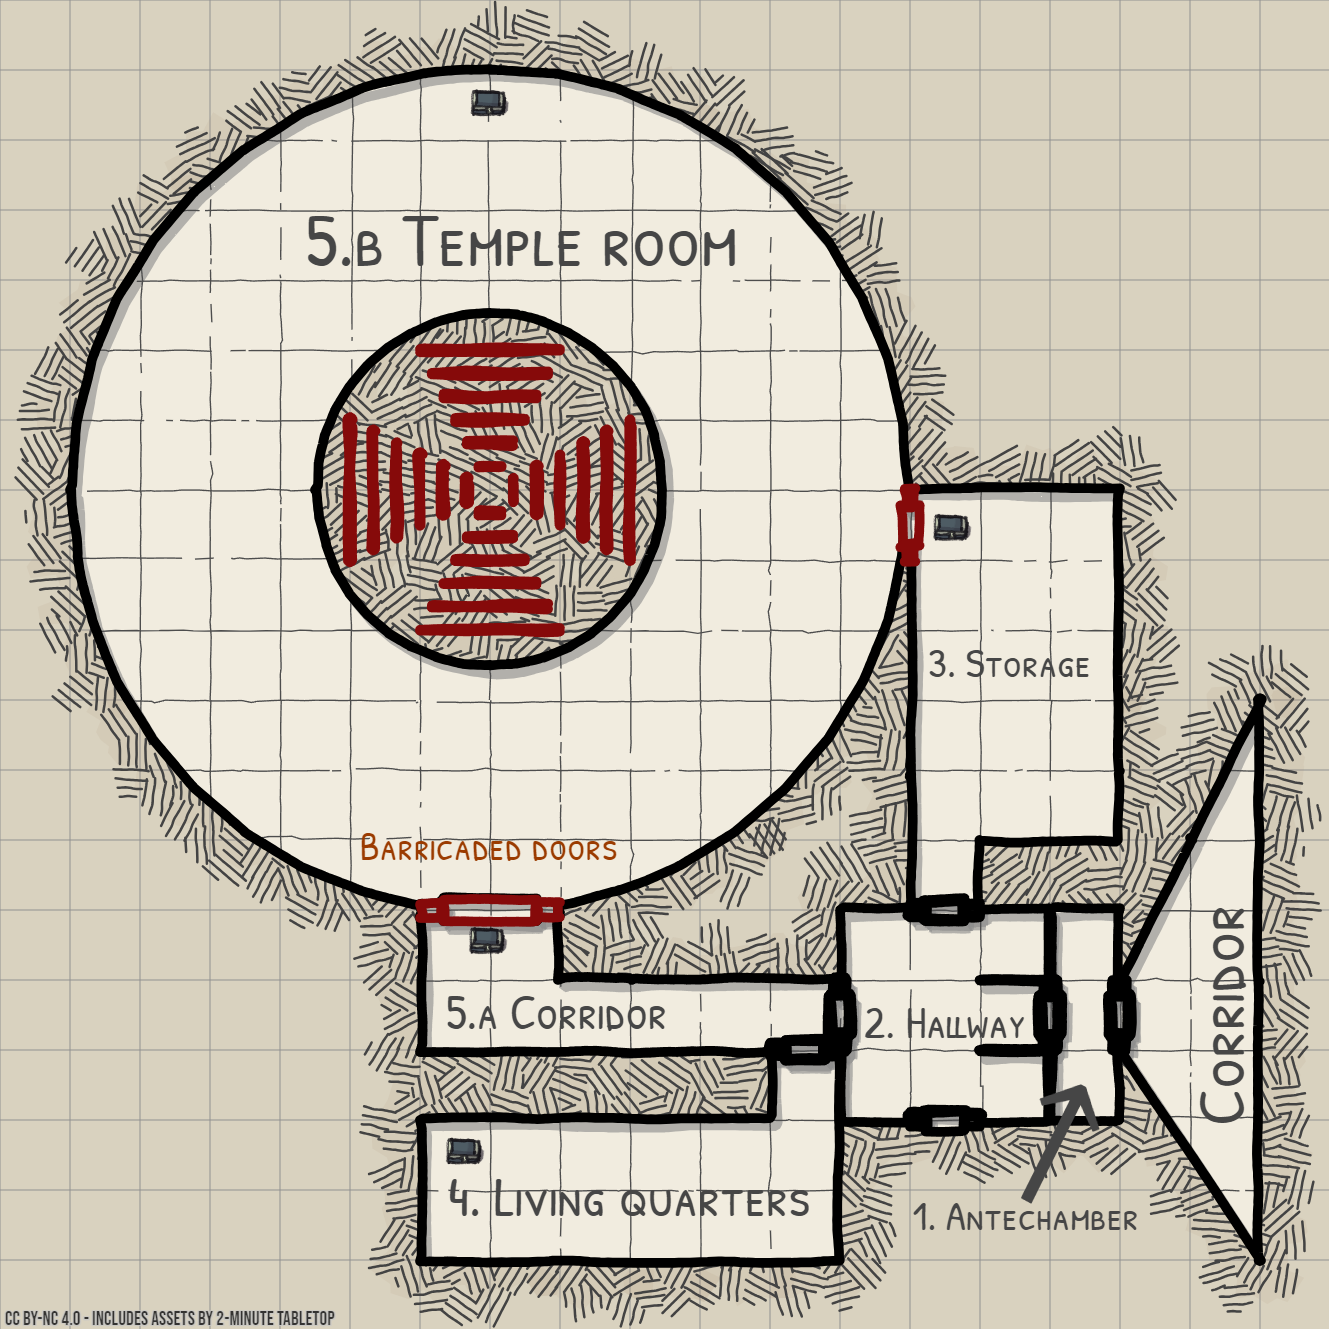
\includegraphics[width=1\textwidth]{img/maps/dm_ruined_temple_map_19x19}

The map was made with: \href{https://probabletrain.itch.io/dungeon-scrawl}{Dungeon Scrawl}.

After another hour of walk, in one corridor the ring points to the wall, but you cannot see any door.
Simply pushing the wall will open a secret door leading to a small antechamber, but as they do,
unless they do it very slowly, a rattling of bones can be heard as the door opens.
Behind the door were hung bones of various creatures on a sinuous string which rattles if the door is opened.
\vfill
\newpage

\DndArea{Antechamber}
The original dwarven stonework of the entrance and the interior are almost crumbled now.
Walls and floors are smeared with filth, blood and dung, there are bones and skulls of various creatures everywhere.
The air is damp, and the smell of rotting flesh mixed with dung is unbearable.

\DndArea{Hallway}
Hallway is dark, smeared by dried blood and dung same as in antechamber.
The repugnant odour fills the air.
It has a high ceiling, which probably collapsed long time ago.

Players may roll perception checks now. \\
Perception DC 15+ reveals a few big bat-like creatures hanging on the ceiling waking up and heading straight at the party.
On failed check \href{https://www.dndbeyond.com/monsters/17023-stirge}{four stirges} will have a surprise round.

\DndArea{Storage}
The storage room is covered with crimson crystalline fungi-like growths.
At the far end of the room, there are few crumbling chests also covered by crystalline mould; there might be something inside.
Moving through means that players are risking to get infected by the mould.
On touch crystalline structure shatters, and splinters may hit the character (DC 12 DEX saving throw).
If the splinter it touches their skin, they will have to make a DC 12 CON save or get infected by \textbf{"Bloodborne Disease"}.

If there is a player who is enjoying healing and herbalism, you can give use this overly detailed description of the disease to help you role-play the symptoms and the cure.\\
Feel free to make it simple.
\begin{DndComment}{Bloodborne Disease}
\begin{itemize}
\item DC 11 Constitution saving throw against disease or becoming poisoned until the disease is cured.
\item Every 24 hours that elapse, the creature must repeat the saving throw, reducing its hit point maximum by 5 (1d10) on a failure.
This reduction lasts until the disease is cured.
The creature dies if the disease reduces its hit point maximum to 0
\end{itemize}

\subsubsection*{Symptoms:}
\begin{itemize}
  \item 1. Early Onset: When a creature comes into contact with the crystallized blood mould, it may initially experience mild symptoms, including fatigue, nausea, and a persistent metallic taste in its mouth.
    \begin{itemize}
      \item Herbs to help: Ginger, Peppermint
    \end{itemize}

  \item 2. Crystalline Skin: Over time, their skin takes on a pallid, translucent appearance, and small, crystalline nodules begin to form on their body, resembling drops of dried blood. These nodules may occasionally burst, releasing spores that further infect the individual.
    \begin{itemize}
      \item Herbs: Aloe Vera, Lavender
    \end{itemize}

  \item 3. Persistent Weakness: As the infection progresses, those afflicted with the Bloodveil Infection grow progressively weaker.
  Their muscles atrophy, and they experience constant lethargy and shortness of breath.
    \begin{itemize}
      \item Herbs to help: Devil's Claw, Ginger, Turmeric, Arnica, Cayenne
    \end{itemize}

  \item 4. Visceral Hallucinations: Sufferers of the disease begin to have vivid and disturbing hallucinations, often
  involving blood, mould, and the presence of malevolent, whispering voices.
  These hallucinations can cause paranoia and extreme psychological distress.

  \item 5. Bleeding Sores: Dark, oozing sores appear on their skin, especially near the site of the initial contact with the blood mould.
  These sores seep a black, viscous fluid that further spreads the infection.


\begin{itemize}
\item Herbs to help: Yarrow, Calendula, Aloe Vera, Witch Hazel
\end{itemize}

\item 6. Horrific Hemorrhages: As the disease worsens, internal bleeding becomes frequent and severe, causing intense pain, dizziness, and eventually leading to organ failure.
\begin{itemize}
\item Herbs to help: Cayne, Yarrow, turmeric
\end{itemize}
\end{itemize}

\subsubsection*{Solution to stop spread}
\begin{itemize}
\item Restrict the blood source.
\item Seal and limit growth - magically or physically seal.
\item Magically - dispel, cure disease, purify water, blessed water, banish, remove curse, purifying spells - some combination of spells or potions.
Anti-fungal agent.
\item Magical protective shields and wards.
\item Extreme temperatures - ray of frost/firebolt can destroy 1 square foot but may disperse spores...
\item Light sensitivity - extreme brightness from a magical lamp, daylight spell stops the spread.
\item Dislikes allicin and organosulfur compounds (garlic), blessed oil, and salt - ideally combined.
\item Sound - Resonant, loud music disrupts crystal growth.
\end{itemize}

\subsubsection*{Natural healing:}
\begin{itemize}
\item Isolation to stop transition
\item Painkillers
\begin{itemize}
  \item alcohol, drugs
\item White Willow Bark (Salix alba)
\end{itemize}
\item Mix of Common herbs to cure symptomps cost ~10s/per day of remedy
\item Antifungal solutions
\begin{itemize}
  \item Garlic, Turmeric (Curcuma), ginger
\end{itemize}
\item Antitoxic solutions
\begin{itemize}
\item Activated Charcoal
\item Cillantro
\item Chlorella
\end{itemize}
\item Combine - rare herbs to promote strength of muscles, blood cleansing, anti-fungoid
\begin{itemize}
\item 50g to mix it
\item (Magical) Silvershade Fern - blood cleansing, circulation, heart functions
\item (Magical) Vitalis Moss - physical enhancer - regenerate muscles
\item (Magical) Serenity Root - anti-fungoid, calms, removes hallucinations
\end{itemize}
\item Extreme temperatures (fever, cold spells on blisters)
\end{itemize}

\subsubsection*{Magical healing:}
\begin{itemize}
\item Potion of lesser restoration
\item Dispel
\item Remove curse
\item Abjuration shield spells somehow improvise
\end{itemize}

\subsubsection*{Origin:}
It can be traced probably to Thanatos, the Belly of Death, layer of Abyss.

\end{DndComment}


Investigation skill check DC 10 while actively looking at the walls and far west corner reveals a potential hidden way.
\begin{DndReadAloud}
Five feet above the floor is a hole leading to another room, but it's covered by the same crimson crystalline mould.
You can hear some kind of growling and guttural language from the other side and see faint flickers of light.
\end{DndReadAloud}
This secret passage leads straight to the main temple room (5.B).

Players can get to the chests and find 3lb of silver (bricks), 24lb of copper ingots.
Every other material that might have been there (food, fabrics or leather) seems to be decayed or destroyed by the mould.
\DndArea{Living quarters}
This room used to be a living quarters as you notice some broken wooden beds and destroyed simple chests.
Fresh blood and fresh dung, some of it on the walls covers the room, and the smell becoming even more aggressive.
Gnawed bones and skulls of various creatures lie scattered around the room.
And you see two tall lizard-like creatures \textbf{(two \href{https://www.dndbeyond.com/monsters/17204-troglodyte}{troglodyte})} eating the legs and hands of a humanoid.
They're aggressive and will attack the party.
When slain players can wade through the filth and in the room and find:
\begin{itemize}
  \item golden ring
  \item golden necklace
  \item 20 gold pieces
\end{itemize}
\DndArea{Temple}
\DndSubArea{Corridor}
\begin{DndReadAloud}
At the end of the corridor, you see a large door leading to a larger room.
The door barricaded from your side, indicates the last futile fight of men lying at the base of the door frame.
The half-eaten bodies (missing hands and legs) of a humans (Lyra's father and his companion).
A ring, almost identical to Lyra's, on a chain hangs from the neck of one of the remains of men with breastplate
with a Lessoir family crest, his scimitar with a blue gemstone in the hilt lies nearby.
You can hear some kind of growling and guttural language from the other side.
\end{DndReadAloud}
In case players didn't visit the living quarters (3.), when troglodytes finish their meal, they will come to the corridor and attack the party.

Players can find few items, by the door:
\begin{itemize}
  \item Breastplate with a Lessoir family crest
  \item scimitar with a blue gemstone in the hilt
  \item short sword
  \item healing potion
  \item magical scroll of first level (choose something players can use ot want ideally)
\end{itemize}
Opening the barricaded door requires a DC 14 STR check or by using some tools to cut through the old door.
\begin{itemize}
  \item Failed check will result in a loud noise attracting the troglodytes inside.
A fiery explosion opens the door, players can make DEX saving throw DC 13 to avoid the 1d10 fire damage (half on success)
  as troglodyte shaman casts a spell on the door.
  Combat starts with \textbf{\href{https://www.dndbeyond.com/monsters/17278-kobold-scale-sorcerer}{troglodyte shaman}}
  and two \textbf{\href{https://www.dndbeyond.com/monsters/17204-troglodyte}{troglodyte warriors}}.
  \item Success means prying the door open with minimal noise.
  \end{itemize}
\DndSubArea{Main Room}\label{subsec:main-teple-room}
Entering a room with a wide hole in the middle reveals a stunning view.
A pinnacle of filthiness and decay, almost unbearable stench fills the room.
Blood dripping from the ceiling above the pit, walls smeared with it.
From the hole, a crimson crystalline mould grows and spreads on the walls towards the east side of the room.
Silgrid or religion check DC 13 reveals that this was a temple to the goddess Shar.

If players came quietly, they might see a lizard-like shaman performing a blasphemous
sacrificial ritual at the far end of the circular room.
An archer in leather armor (unconscious), lying on a flat stone altar as the shaman chanting in guttural voice.
If interrupted, combat starts with \href{https://www.dndbeyond.com/monsters/17278-kobold-scale-sorcerer}{troglodyte shaman}
and two \href{https://www.dndbeyond.com/monsters/17204-troglodyte}{troglodyte warriors}.
Unless players react immediately, the shaman finishes the ritual and the archer dies.
If rescued, the archer thanks the party and offers his help to get out of this place.
Improvise his story about how he came for one last treasure hunt with his companions (including Lyra's father),
as the troglodytes ambushed them.

If archer dies, they can loot his body, or if rescued, he will give them:
\begin{itemize}
  \item leather armor
  \item shortbow
  \item 20 arrows
\end{itemize}
Somewhere in the room, players can find a small black box.
It's locked with magical lock.
Each lock is decorated with a different animal.
\begin{DndReadAloud}
On the top of the box, there are four keyholes, each with a different animal decoration.\\
The first lock has a dog, the second has two mice, the third has three cats, and the fourth has a spider.\\
You have four keys with it on a chain.
\end{DndReadAloud}
Players have to look at the keys and count the teeth to find the right key for each lock, each word represents the
number of teeth of the keys.
If they fail to insert the right key, a monster corresponding to the wrong slot will pop up.

Four locks
\begin{itemize}
\item 3 letters; Dog; summons \href{https://www.dndbeyond.com/monsters/16809-blink-dog}{a blink dog}
\item 4 letters; Mice (two mice); summons \href{https://www.dndbeyond.com/monsters/16976-panther}{two panthers}
\item 5 letters; snake; summons \href{https://www.dndbeyond.com/monsters/16890-giant-poisonous-snake}{a giant poisonous snake}
\item 6 letters; spider; summons \href{https://www.dndbeyond.com/monsters/16895-giant-spider}{a giant spider}
\end{itemize}

If solved, the box opens and reveals a document \textbf{claim of a "Trollskull Mansion"} which enables the owner to
claim the building for a fee at Waterdeep office.\\
Trollskull mansion is a historical building and haunted house in the North Ward of Waterdeep.
If no player got the idea to return the remains of Lyra's father to Lyra, Norman will suggest it.
Characters should probably take a short rest to restore some hit points.

\subsubsection{On the way back}
As the party leaving the ruined temple, an armored thug bars the doorway leading from the antechamber to the Undermountain tunnel.
From behind him a familiar voice of Harold's rival, Ray Cox, could be heard.
\begin{DndReadAloud}
"Haha, now give us what you stole, this is my territory!"
\end{DndReadAloud}
It's an obvious lie, but Ray is trying to intimidate the party, to drop weapons, loot, everything they wear and carry with a promise to spare their lives.
If players refuse, combat starts with three to four \href{https://www.dndbeyond.com/monsters/17035-thug}{thugs} and
Ray Cox (\href{https://www.dndbeyond.com/monsters/17021-spy}{spy}), at this point characters should be in a bad shape and should lose this fight.
Try to use thugs as front line and take advantage of their pack tactics ability.
Position them around the door and use Ray Cox (spy) as a ranged attacker rogue.
Do as many sneak attacks as possible, hide as a bonus action each turn and attack with an advantage.
Thugs and Ray will not kill the party but knock them out.

When players lose the fight.
\begin{itemize}
  \item They will take all their loot and weapons.
  \item Elf adventurers, Shalana (and her companions) will, tend to their wounds and lead them back to the Yawning Portal.
  Party can take a short or long rest while elves are watching over them.
  Shalana will require a favour in the future.
  \item They realize that Norman (or the NPC in the party) was kidnapped.
\end{itemize}

If players win, they can loot the thugs and Ray Cox.
\begin{itemize}
  \item Ray will say that he was hired by Arnold Fenxis.
  \item Loot sending stones, 30 gold pieces, hand crossbow, short sword, 2x heavy crossbows, 10x bolts, 2x maces
\end{itemize}



\subsection{Haunted House}\label{subsec:haunted-house}
\lipsum[1]

\subsection{Swarm of Bats}\label{subsec:swarm-of-bats}
\lipsum[1]

\vfill
\newpage

\chapter{Maps}\label{ch:maps}
\section{Ruined Temple player map}\label{sec:ruined-temple}
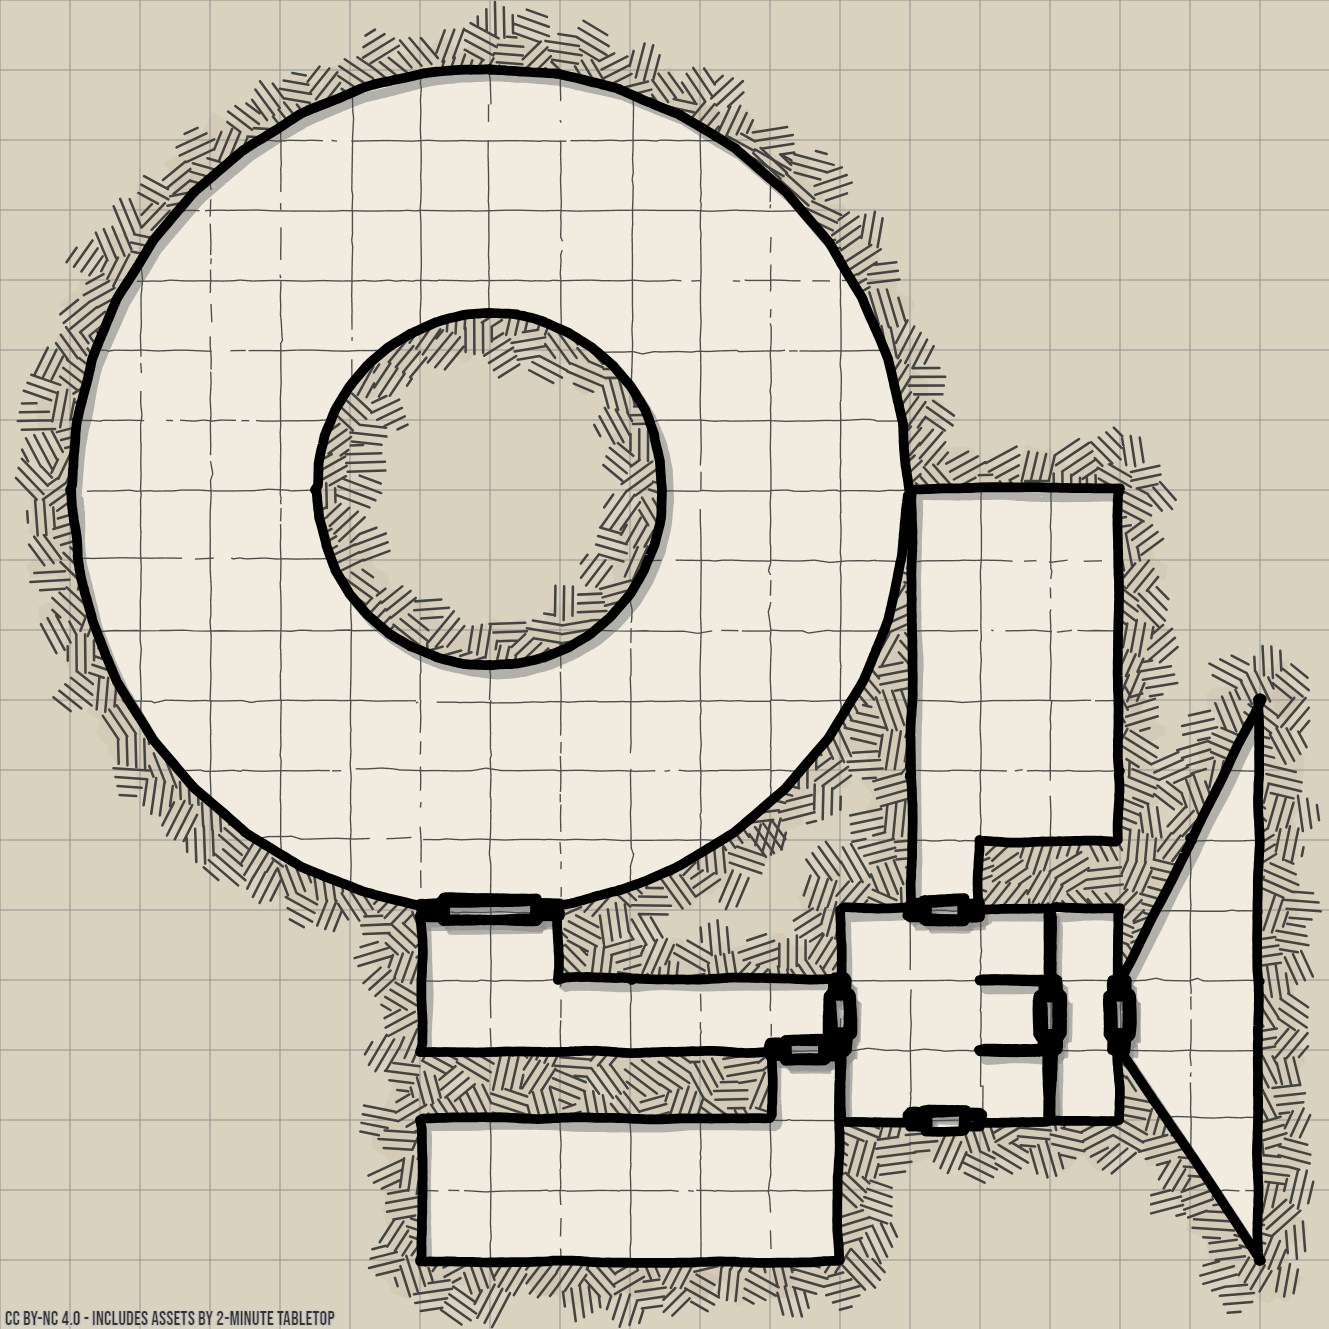
\includegraphics[width=1\textwidth]{img/maps/ruined_temple_map_19x19}
Author: Tomáš Fanta

\subsection* {Printable version}
Print, cut and glue the map together.
\includepdf[pages=-]{img/maps/ruined_temple_print.pdf}

\vfill
\newpage
\section{Trollskull Tavern player map}\label{sec:trollskull-tavern-player-map}
Recreated by me from the original from the Dragonheist module, with some adjustments and secret bar addition in the basement.
\subsection* {Printable version}
Each page is one floor.
\includepdf[pages=-]{img/maps/trollskull_print.pdf}


\section{Knight and Shadow Tavern player map}\label{sec:knight-and-shadow-tavern}
In case you need a map for the Knight and Shadow tavern.
Author: Tomáš Fanta
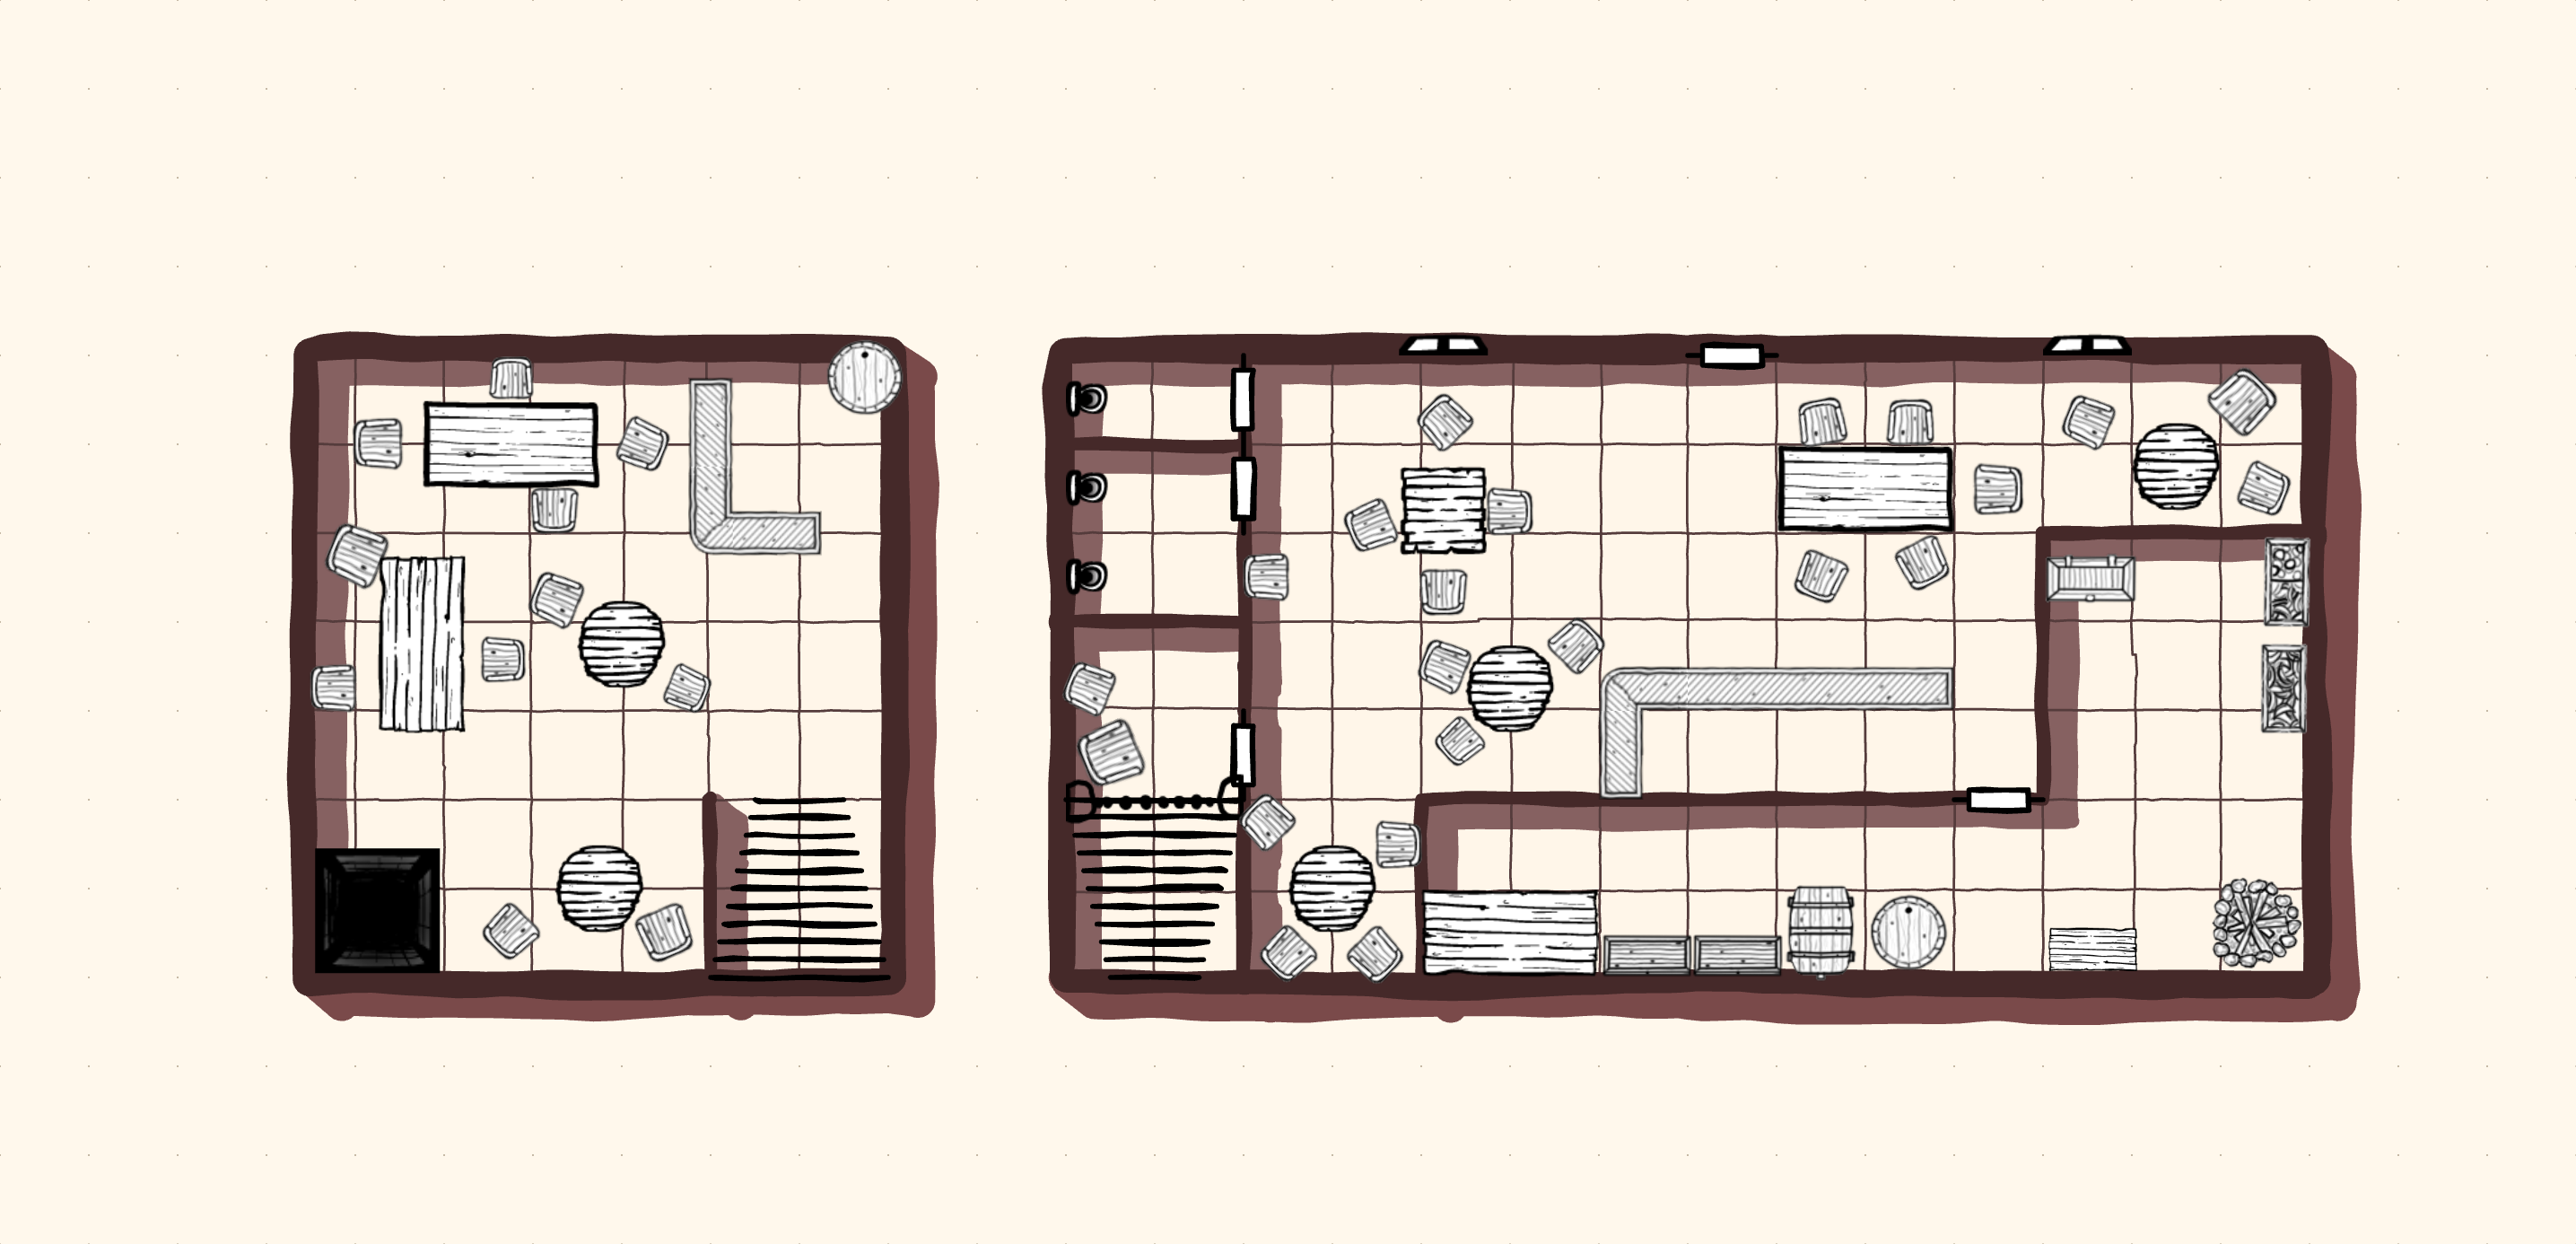
\includegraphics[width=1\textwidth]{img/maps/knight_and_shadow_tavern}

\vfill
\newpage
\chapter{Character Sheets}\label{ch:charactersheets}

\end{document}

